\chapter{Processazione}

\section{Introduzione}
Dopo la rimozione di un campione di tessuto dal paziente, una serie di processi fisici e chimici deve essere effettuata per garantire che i preparati microscopici finali siano di qualità diagnostica.  
I tessuti vengono esposti a una sequenza di reagenti che li fissano, disidratano, chiarificano e infiltrano. Infine, il tessuto viene inglobato in un mezzo che ne fornisce il supporto per il taglio al microtomo.

La qualità della conservazione strutturale dei componenti del tessuto dipende dalla scelta dei tempi di esposizione ai reagenti durante la processazione. Ogni fase — dalla selezione del campione alla scelta dei reagenti e protocolli, fino alla colorazione e diagnosi finale — è cruciale.

La produzione di preparati di qualità diagnostica richiede competenze che si affinano con l’esperienza. Con lo sviluppo di nuove tecnologie e strumentazioni, il ruolo del laboratorio di istologia continua a evolversi, migliorando la standardizzazione, la produttività e l’uso efficiente delle risorse.  

Questo capitolo fornirà una panoramica dei passaggi fondamentali e dei reagenti impiegati nella preparazione dei tessuti per la valutazione microscopica.



\section{Principi della processazione dei tessuti}
La processazione ha lo scopo di rimuovere l’acqua estraibile dal tessuto, sostituendola con un mezzo di supporto solido che ne permetta il taglio al microtomo senza danneggiare o distorcere le strutture cellulari.

\subsection{Fattori che influenzano la velocità di processazione}
Durante l’immersione del tessuto nei fluidi, si verifica uno scambio tra il liquido intracellulare e quello esterno. La velocità di questo scambio dipende da vari fattori (Figura \ref{fig:factors-penetrazione}):

\begin{itemize}
    \item Agitazione del fluido;
    \item Temperatura (calore);
    \item Viscosità del reagente;
    \item Applicazione di pressione o vuoto.
\end{itemize}


\begin{figure}[htbp]
  \centering
  \begin{tikzpicture}[
      box/.style={rectangle, draw, rounded corners=2mm, minimum width=36mm, minimum height=7mm, align=center, font=\small},
      small/.style={font=\footnotesize},
      arr/.style={{Stealth[length=3mm,width=2mm]}-{Stealth[length=3mm,width=2mm]}, line width=0.6pt}
    ]
    % core tissue
    \node[draw, circle, minimum size=22mm, align=center] (tissue) {Campione\\(tessuto)};
    % factors around
    \node[box, above left=10mm and 26mm of tissue] (agit) {Agitazione \\ (meccanica / flusso)};
    \node[box, above right=10mm and 26mm of tissue] (heat) {Calore \\ (\textless{} 45°C)};
    \node[box, below left=10mm and 26mm of tissue] (visc) {Viscosità \\ (reagente)};
    \node[box, below right=10mm and 26mm of tissue] (vac) {Vuoto/Pressione \\ (max 50,79 kPa)};
    % arrows to tissue
    \draw[->, line width=0.6pt] (agit) -- (tissue);
    \draw[->, line width=0.6pt] (heat) -- (tissue);
    \draw[->, line width=0.6pt] (visc) -- (tissue);
    \draw[->, line width=0.6pt] (vac) -- (tissue);

  \end{tikzpicture}
  \caption{Fattori principali che influenzano la velocità di penetrazione e scambio dei reagenti nel tessuto.}
  \label{fig:factors-penetrazione}
\end{figure}

\subsubsection{Agitazione}
L’agitazione favorisce il flusso di soluzione fresca intorno al tessuto. I processatori automatici utilizzano movimenti oscillatori o sistemi di flusso pressurizzato per migliorare l’efficienza, riducendo fino al 30\% i tempi complessivi di processazione.

\subsubsection{Calore}
L’aumento della temperatura accelera la penetrazione dei reagenti, ma un eccesso di calore (oltre i 45°C) può danneggiare le strutture cellulari o interferire con successive colorazioni immunoistochimiche.

\subsubsection{Viscosità}
La viscosità misura la resistenza di un fluido al flusso: soluzioni meno viscose (a molecole più piccole) penetrano più rapidamente. La paraffina fusa, a temperatura controllata, ha una bassa viscosità e permette un’infiltrazione efficiente.

\subsubsection{Vuoto}
L’applicazione del vuoto facilita l’infiltrazione e rimuove bolle d’aria dai tessuti porosi. Non deve superare i 50,79~kPa per evitare danni strutturali.

Questi fattori sono facilitati nella camera dei processatori automatici per ottimizzare la qualità e la velocità della processazione (Figura \ref{fig:camera_vuota} ).

\begin{figure}[htbp]
    \centering
    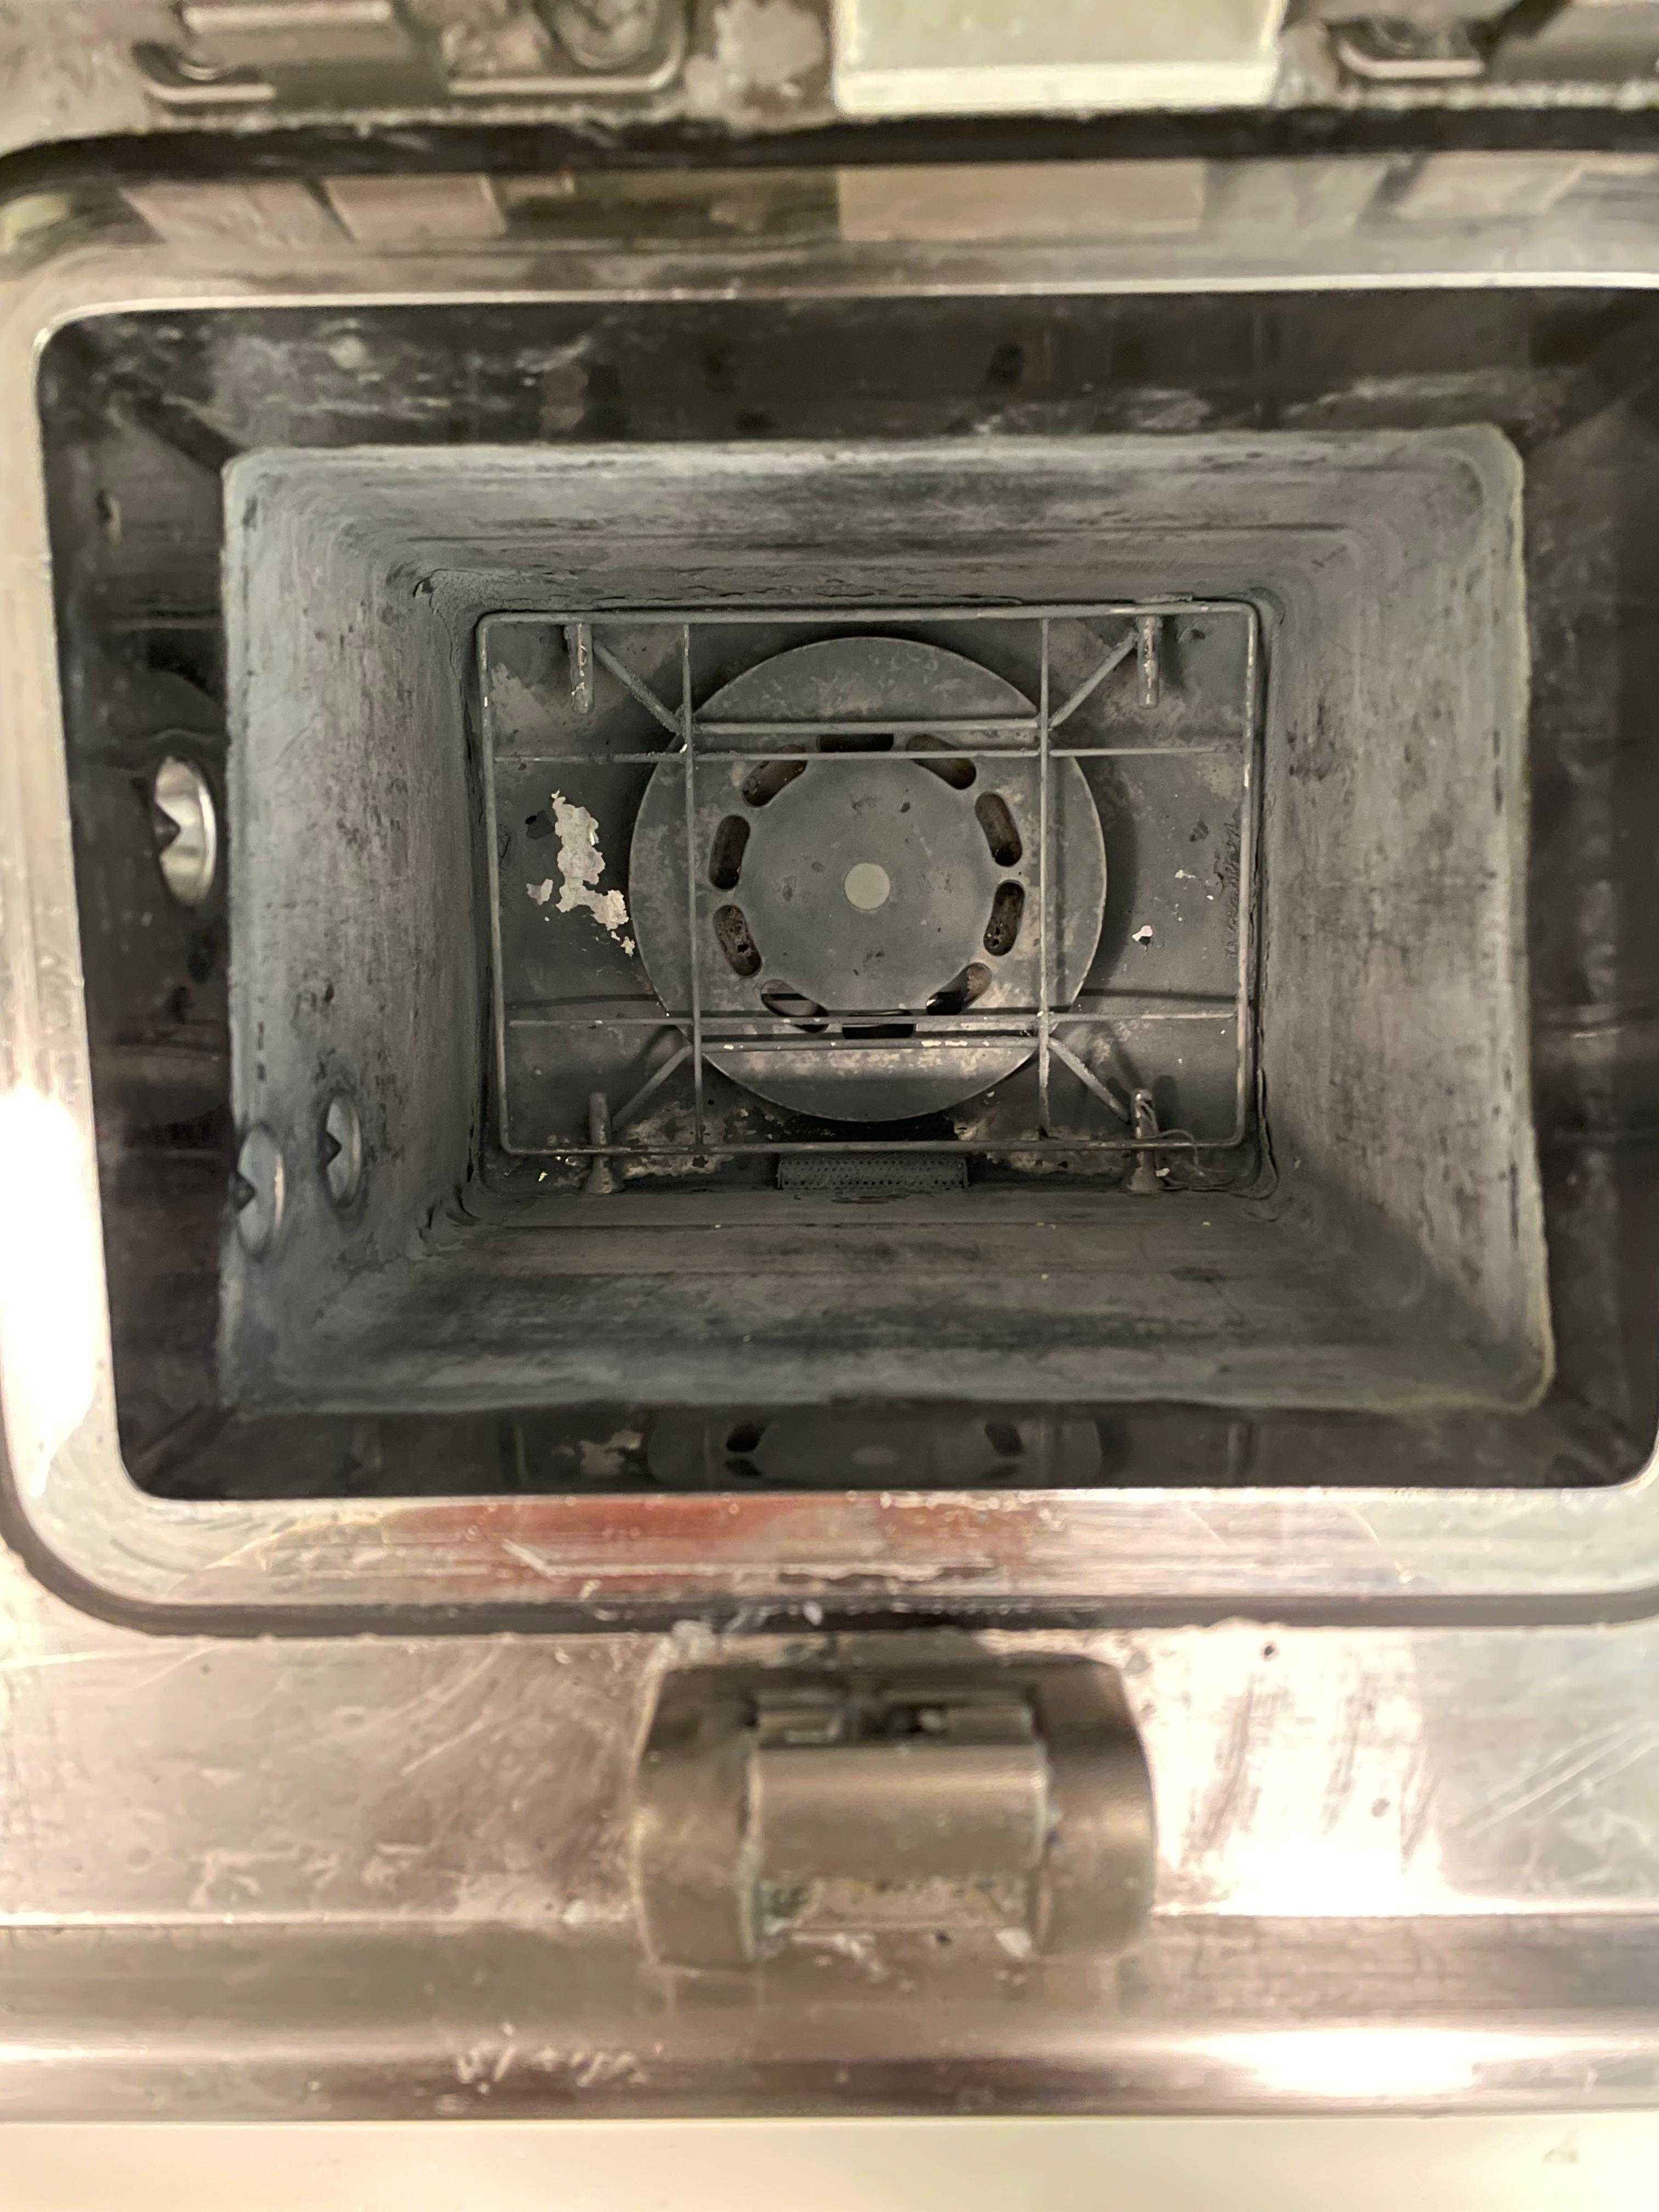
\includegraphics[width=0.75\textwidth]{processazione_camera_vuota}
    \caption{La camera del processatore automatico.}
    \label{fig:camera_vuota}
\end{figure}

\section{Fasi della processazione dei tessuti}
\begin{enumerate}
    \item \textbf{Fissazione}: stabilizza e indurisce il tessuto minimizzando la distorsione cellulare;
    \item \textbf{Disidratazione}: rimozione graduale dell’acqua e dei fissativi acquosi;
    \item \textbf{Chiarificazione}: sostituzione dei fluidi disidratanti con solventi intermedi;
    \item \textbf{Infiltrazione}: impregnazione del tessuto con un mezzo di supporto (es. paraffina);
    \item \textbf{Inclusione}: orientamento del campione nel mezzo e solidificazione.
\end{enumerate}

% \textbf{Figura suggerita 3:}  
% \textit{Diagramma a flusso della processazione istologica.}  
% (Didascalia: “Le cinque fasi principali della processazione dei tessuti: fissazione, disidratazione, chiarificazione, infiltrazione e inclusione.”)



\section{Fissazione}
L’obiettivo principale è preservare le cellule e i componenti tissutali con la minima distorsione possibile.  
La fissazione stabilizza le proteine, rendendo il tessuto resistente all’autolisi e alla decomposizione. Deve essere completata prima di avviare le fasi successive della processazione.



\section{Disidratazione}
La disidratazione elimina l’acqua libera e i fissativi acquosi. Deve essere graduale per evitare artefatti dovuti a differenze di concentrazione troppo elevate.

\subsection{Agenti disidratanti}
Tra i più utilizzati:
\begin{itemize}
    \item Etanolo;
    \item Alcol denaturato (spirito metilato industriale);
    \item Metanolo;
    \item Isopropanolo;
    \item Butanolo;
    \item Acetone.
\end{itemize}

% --- Tabelle ---
% Tabella 1: Confronto agenti disidratanti
\begin{table}[htbp]
  \centering
  \caption{Confronto tra i principali agenti disidratanti}
  \label{tab:disidratanti}
  \begin{adjustbox}{max width=\textwidth}
  \begin{tabular}{@{}lllll@{}}
    \toprule
    \textbf{Reagente} & \textbf{Velocità} & \textbf{Effetto sul tessuto} & \textbf{Tossicità / Note} & \textbf{Uso tipico} \\
    \midrule
    Etanolo (70--95--100\%) & \emph{Moderata -- rapida} & Rischio di indurimento se eccesso & Moderata; soggetto a tassazione & Routine, EM \\
    Alcol denaturato & Simile all'etanolo & Simile all'etanolo & Contiene metanolo/isopropanolo & Alternativa economica \\
    Metanolo & Rapida & Può indurire & Alta tossicità & Sostituto in protocolli specifici \\
    Isopropanolo & Moderata & Minore indurimento & Minore tossicità rispetto al metanolo & Processazione a microonde \\
    Butanolo & Lenta & Meno restringimento & Meno comune & Istologia vegetale/animale \\
    Acetone & Molto rapida & Può causare fragilità & Infiammabile, volatile & Rimozione lipidi, procedure rapide \\
    \bottomrule
  \end{tabular}
  \end{adjustbox}
\end{table}

\subsection{Additivi}
Il fenolo (4\%) può essere aggiunto all’etanolo al 95\% per ammorbidire tessuti duri (tendini, unghie, cheratina). Alternativamente, si può usare una miscela glicerolo-alcol.

\subsection{Solventi universali}
Reagenti come dioxano, tetraidrofurano e butanolo terziario hanno funzioni sia disidratanti che chiarificanti, ma sono tossici e poco usati oggi.



\section{Chiarificazione}
Gli agenti chiarificanti sostituiscono i fluidi disidratanti, rendendo i tessuti traslucidi e pronti per l’infiltrazione. Sono idrocarburi miscibili sia con i solventi organici che con la paraffina.

\subsection{Criteri di scelta}
Un buon chiarificante deve:
\begin{itemize}
    \item Penetrare rapidamente;
    \item Rimuovere facilmente l’alcol residuo;
    \item Essere sostituito agevolmente dalla paraffina fusa;
    \item Non danneggiare il tessuto;
    \item Avere bassa tossicità e infiammabilità;
    \item Essere economico e smaltibile in sicurezza.
\end{itemize}

\subsection{Agenti chiarificanti comuni}
\begin{description}
    \item[Xilene:] rapido, efficace ma tossico; ideale per blocchi sottili (<5 mm).  
    \item[Toluene:] meno dannoso, ma più volatile.  
    \item[Cloroformio:] più lento, adatto a tessuti spessi e al SNC, ma tossico.  
    \item[Sostituti dello xilene:] idrocarburi alifatici con volatilità variabile.  
    \item[Oli di agrumi (limonene):] non tossici ma odorosi e non riciclabili.
\end{description}
% Tabella 2: Confronto chiarificanti
\begin{table}[htbp]
  \centering
  \caption{Confronto tra i principali agenti chiarificanti}
  \label{tab:chiarificanti}
  \begin{adjustbox}{max width=\textwidth}
  \begin{tabular}{@{}lllll@{}}
    \toprule
    \textbf{Reagente} & \textbf{Penetrazione} & \textbf{Compatibilità paraffina} & \textbf{Tossicità / Sicurezza} & \textbf{Note operative} \\
    \midrule
    Xilene & Rapida & Ottima & Tossico, infiammabile & Standard di laboratorio, riciclabile \\
    Toluene & Rapida & Buona & Infiammabile, volatile & Alternativa allo xilene \\
    Cloroformio & Lenta & Buona & Altamente tossico, non infiammabile & Usato in SNC e tessuti spessi \\
    Sostituti xilene (alifatici) & Variabile & Variabile & Generalmente meno aromatici & Alcuni sono meno volatili, attento alla contaminazione cera \\
    Limonene / oli agrumi & Buona & Problemi oleosi & Minore tossicità acuta, sensibilizzanti & Forte odore; non riciclabile \\
    \bottomrule
  \end{tabular}
  \end{adjustbox}
\end{table}



\section{Infiltrazione e inclusione}

\subsection{Paraffina}
La cera paraffinica è il mezzo di infiltrazione e inclusione più diffuso. È composta da idrocarburi a catena lunga con punto di fusione tra 47 e 64°C.  
Durante l’infiltrazione, la paraffina liquida permea il tessuto; raffreddandosi, forma una matrice solida che ne preserva la struttura.

% \textbf{Figura suggerita 6:}  
% \textit{Sezione schematica del tessuto durante l’infiltrazione in paraffina.}  
% (Didascalia: “Penetrazione della cera paraffinica nelle cavità cellulari e solidificazione.”)

\subsection{Mezzi alternativi}
Quando la paraffina non è adatta (per tessuti lipidici, fragili o soggetti a calore), si possono impiegare altri mezzi:
\begin{itemize}
    \item \textbf{Resina:} per sezioni ultrafini e microscopia elettronica;
    \item \textbf{Agar:} per piccoli frammenti friabili (doppia inclusione);
    \item \textbf{Gelatina:} per sezioni intere di organi o sezioni congelate;
    \item \textbf{Celloidina:} raramente usata oggi, in neuropatologia.
\end{itemize}



% \section{Inclusione in paraffina}
% L’inclusione prevede l’incapsulamento dei campioni orientati nel mezzo fuso. Dopo il raffreddamento rapido su piastra fredda, si ottiene un blocco compatto e omogeneo.

% \textbf{Figura suggerita 7:}  
% \textit{Fotografia o schema del centro di inclusione modulare.}  
% (Didascalia: “Componenti principali di un centro di inclusione: dispensatore di paraffina, piastra fredda e area riscaldata.”)



\section{Processazione automatizzata dei tessuti}
Il principio fondamentale consiste nello scambio sequenziale di fluidi per tempi predefiniti in condizioni controllate.  
Le apparecchiature moderne includono:
\begin{itemize}
    \item Processatori chiusi;
    \item Processatori a microonde;
    \item Sistemi a flusso continuo.
\end{itemize}

\subsection{Processatori a microonde}
I forni a microonde specifici per istologia riducono i tempi da ore a minuti grazie al riscaldamento uniforme del campione. Hanno controllo preciso di temperatura, tempo e ventilazione, ma richiedono attenzione e costi elevati.

\subsection{Vantaggi delle nuove tecnologie}
\begin{itemize}
    \item Programmi personalizzabili in base al tipo di tessuto;
    \item Tempi ridotti e migliore qualità;
    \item Contenimento dei fumi e risparmio di reagenti;
    \item Maggiore sicurezza e sostenibilità ambientale.
\end{itemize}

% \textbf{Figura suggerita 8:}  
% \textit{Diagramma comparativo tra processazione tradizionale e a microonde.}  
% (Didascalia: “Confronto tra i tempi e la qualità della processazione con metodi convenzionali e a microonde.”)



\section{Riassunto}
La processazione dei campioni chirurgici e bioptici è un passaggio chiave per la preparazione dei tessuti alla valutazione microscopica.  
Le fasi principali comprendono:
\begin{itemize}
    \item Fissazione, 
    \item disidratazione, 
    \item chiarificazione e 
    \item infiltrazione;
\end{itemize}
La qualità del preparato dipende da variabili fisiche (agitazione, calore, viscosità, vuoto) e dalla corretta applicazione dei protocolli.  
L’introduzione di tecnologie automatizzate e processatori a microonde ha ridotto i tempi, aumentato la standardizzazione e migliorato la qualità dei risultati diagnostici.
Il passaggio successivo alla processazione è l'inclusione in paraffina.

